\subsection{Convolutional NN - Zusatz}


\begin{frame}
\frametitle{Anfänge}

\begin{itemize}
\item Yann LeCun: erstes Modell zum Erkennen von Handschrift
\item \emph{Verwendung von MNIST database of handwritten digits}
\begin{itemize}
	\item 60.000 Trainingsdatensätze
	\item 10.000 zum Berechnen des Fehlers
\end{itemize}
\end{itemize}

\begin{figure}
	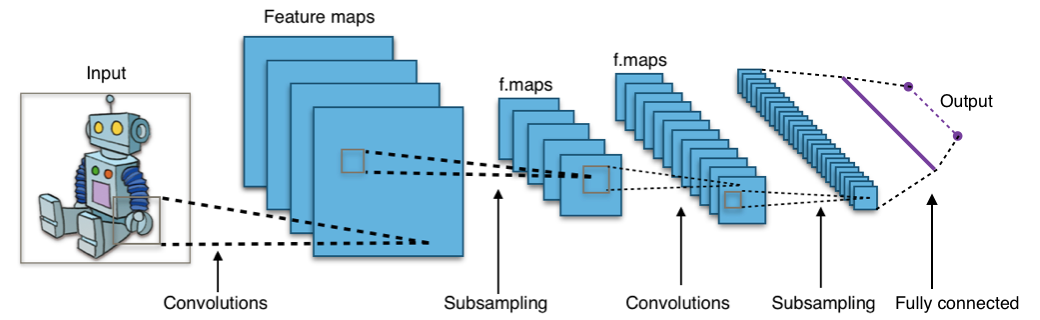
\includegraphics[width=.9\linewidth]{./aktuelleEntwicklung/convolutionalNN/img/cnn_overview_alpha}
\end{figure}


\note[item]{Pioniere, fr. Informatiker Yann LeCun}
\note[item]{Bekannteste Ausarbeitung über CNN für Handschriften}
\note[item]{\emph{Verwendung von MNIST database of handwritten digits}
\begin{itemize}
	\item 60.000 Trainingsdatensätze
	\item 10.000 zum Berechnen des Fehlers
    \item unterschiedliche Personen für Trainings- und Evaluierungsdatensätze
\end{itemize}}

\note[item]{soll erkennen ob ein Bild zu einer (oder mehreren) bestimmten Klasse(n) gehört
\begin{itemize}
    \item von \emph{low-level} Eigenschaften auf komplexe Formen schließen
\end{itemize}}

\note[item]{Covolutional NN: zwei wesentliche Komponenten
\begin{itemize}
    \item \emph{Convolutional layer}: Filter
    \item \emph{Pooling Layer}: Aggregations-Schichten
    \item wiederholen sich abwechselnd
\end{itemize}}

\end{frame}



\begin{frame}
\frametitle{Filter}


\begin{itemize}
\item Generell

\begin{itemize}
	\item Besitzt feste Pixelgröße (\emph{Kernelsize}) \& Schrittweite
	\item Scannt Bild zeilenweise
	\item \emph{Padding} legt Verfahren für Rand des Bildes fest
	\item Ausgabe wird \emph{activation} oder \emph{feature map} genannt
\end{itemize}

\item Praxis
\begin{itemize}
	%\item \emph{Convolutional Layer} mit 32 oder 16 Bit
	\item Jeder Filter generiert eigene Ausgabematrix
	\item Nächster Convolutional Layer verwendet Ausgabematrizen als Input
	\item Ausgabe wird in \emph{Pooling Layer} gesteckt
\end{itemize}

\end{itemize}


\note[item]{Bsp. Filter 2 x 2, Schrittweite: 2 - führt zu Halbierung der InputMatrix
\begin{itemize}
    \item Im Bsp. hängen immer 4 Pixel an einem Filter, die Eingabematrix wird gefaltet (convolute)
\end{itemize}}

\note[item]{Filter generieren eigene Ausgabematrix}
\note[item]{Filter können auch auf Filter folgen}
\note[item]{von Filtern generierte Ausgaben werden auch \emph{activation map} oder \emph{feature map} genannt}

\end{frame}

